
Outline(TODO): In this chapter I will describe the fundamentals of blockchain technology. I will also briefly describe Graph databases and Rust since they'll be used in this thesis.

\section{Cryptographic background}

\subsection{Hash Functions}

A \textit{Hash Function} is a function that deterministically maps an input message $m$ into an output $O=H(m)$ that has a fixed length. $O$ is often called \textit{digest} or simply the \textit{hash of m}.\

\textit{Cryptographic hash functions} (CHF) is a family of hash functions used in many information security applications, such as digital signatures. They are defined as hash functions that satisfy the following properties:

\begin{enumerate}
    \item Efficiency: given a message $m$ it's computationally quick to calculate its digest $H(m)$.
    \item Pre-image resistance: given the digest $H(m)$ it's computationally infeasible to find $m$. $H$ is a one way function.
    \item Second pre-image resistance: given a message $m$ and its digest $H(m)$ it is computationally infeasible to find another message $m'$ such that $H(m)=H(m')$.
\end{enumerate}

This is also the formal definition of One Way Hash Function (OWHF) given by Merkle~\cite{chf}. \

In addition to these three properties, a CHF can also be \textit{collision resistant}. This last property implies that it's computationally infeasible to find two messages $(m,m')$ -- with $m\neq m'$ -- such that $H(m)=H(m')$. A hash function that satisfy this property is called Collision Resistant Hash Function (CRHF).

Hash functions are one of the fundation layers of the concept of blockchain. Typically, eachprotocol decides a cryptographic hash function that is used everytime hashing is needed. Bitcoin uses SHA-256, while Ethereum uses KECCAK-256, a more recent alternative~\cite{bitcoin,Ethereum}.

\subsection{Hash chains}

A hash chain is the sequential application of a cryptographic hash function to a message $m$. For example, $H(H(H(H(H(m)))))$ is a hash chain of length five applied to the string $m$ using the cryptographic hash function $H$, it can be shortened as $H^5(m)$. Image \ref{fig:hash-chain-1} visualize this idea.

\begin{figure}[H]
  \centering
  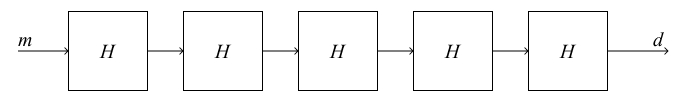
\includegraphics[width=1\textwidth]{Figures/background/hashchain_1.jpg}
  \caption[Hash chain]{}
  \label{fig:hash-chain-1}
\end{figure}

This concept was proposed by Lamport as a way to securely store passwords on servers~\cite{hashchain}. In his proposed protocol, the server just stores $H^n(p)$, where $p$ is the password and $n$ is relatively big number (for example, 1000). When the user wants to authenticate, she sends $H^{n-1}(p)$ and the server computes $H(H^{n-1}(p))$ and checks if it corresponds to $H^n(p)$. If this check succeeds, the user is authenticated and the server replace the stored value with $H^{n-1}(p)$. Next time she wants to authenticate again, she'll need to send $H^{n-2}(p)$ and this value will be checked against the previously sent digest $H^{n-1}(p)$. In this protocol, even if the transmission or the storage of the password is not secure, the user is safe.

Blockchain technology uses this idea to form the immutable chain of blocks: each block contains the hash of the previous one. Modifying a block would result in changing its hash, this would break the chain since all the following blocks would have to be recomputed, changing each digest. As shown in \ref{fig:hash-chain-2}, it's a slightly different concept than the plain hash chain, since on each step, the hashing is done on the previous digest linked to raw data of the current block, so $d_{n}=H(b_n~||~d_{n-1})$

\begin{figure}[H]
  \centering
  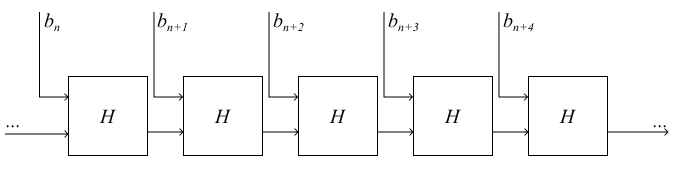
\includegraphics[width=1\textwidth]{Figures/background/hashchain_2.jpg}
  \caption[Hash chain in blockchain]{}
  \label{fig:hash-chain-2}
\end{figure}

\subsection{Merkle trees}

A Merkle tree is a data structure that generalizes the hash chain to efficiently prove membership of data. It's a binary tree in which each leaf node represents the hash of data, while intermediate nodes are computed as the hash of the two child nodes. Figure \ref{fig:merkle-tree} is an example of a Merkle tree with 4 leaf nodes.

\begin{figure}[H]
  \centering
  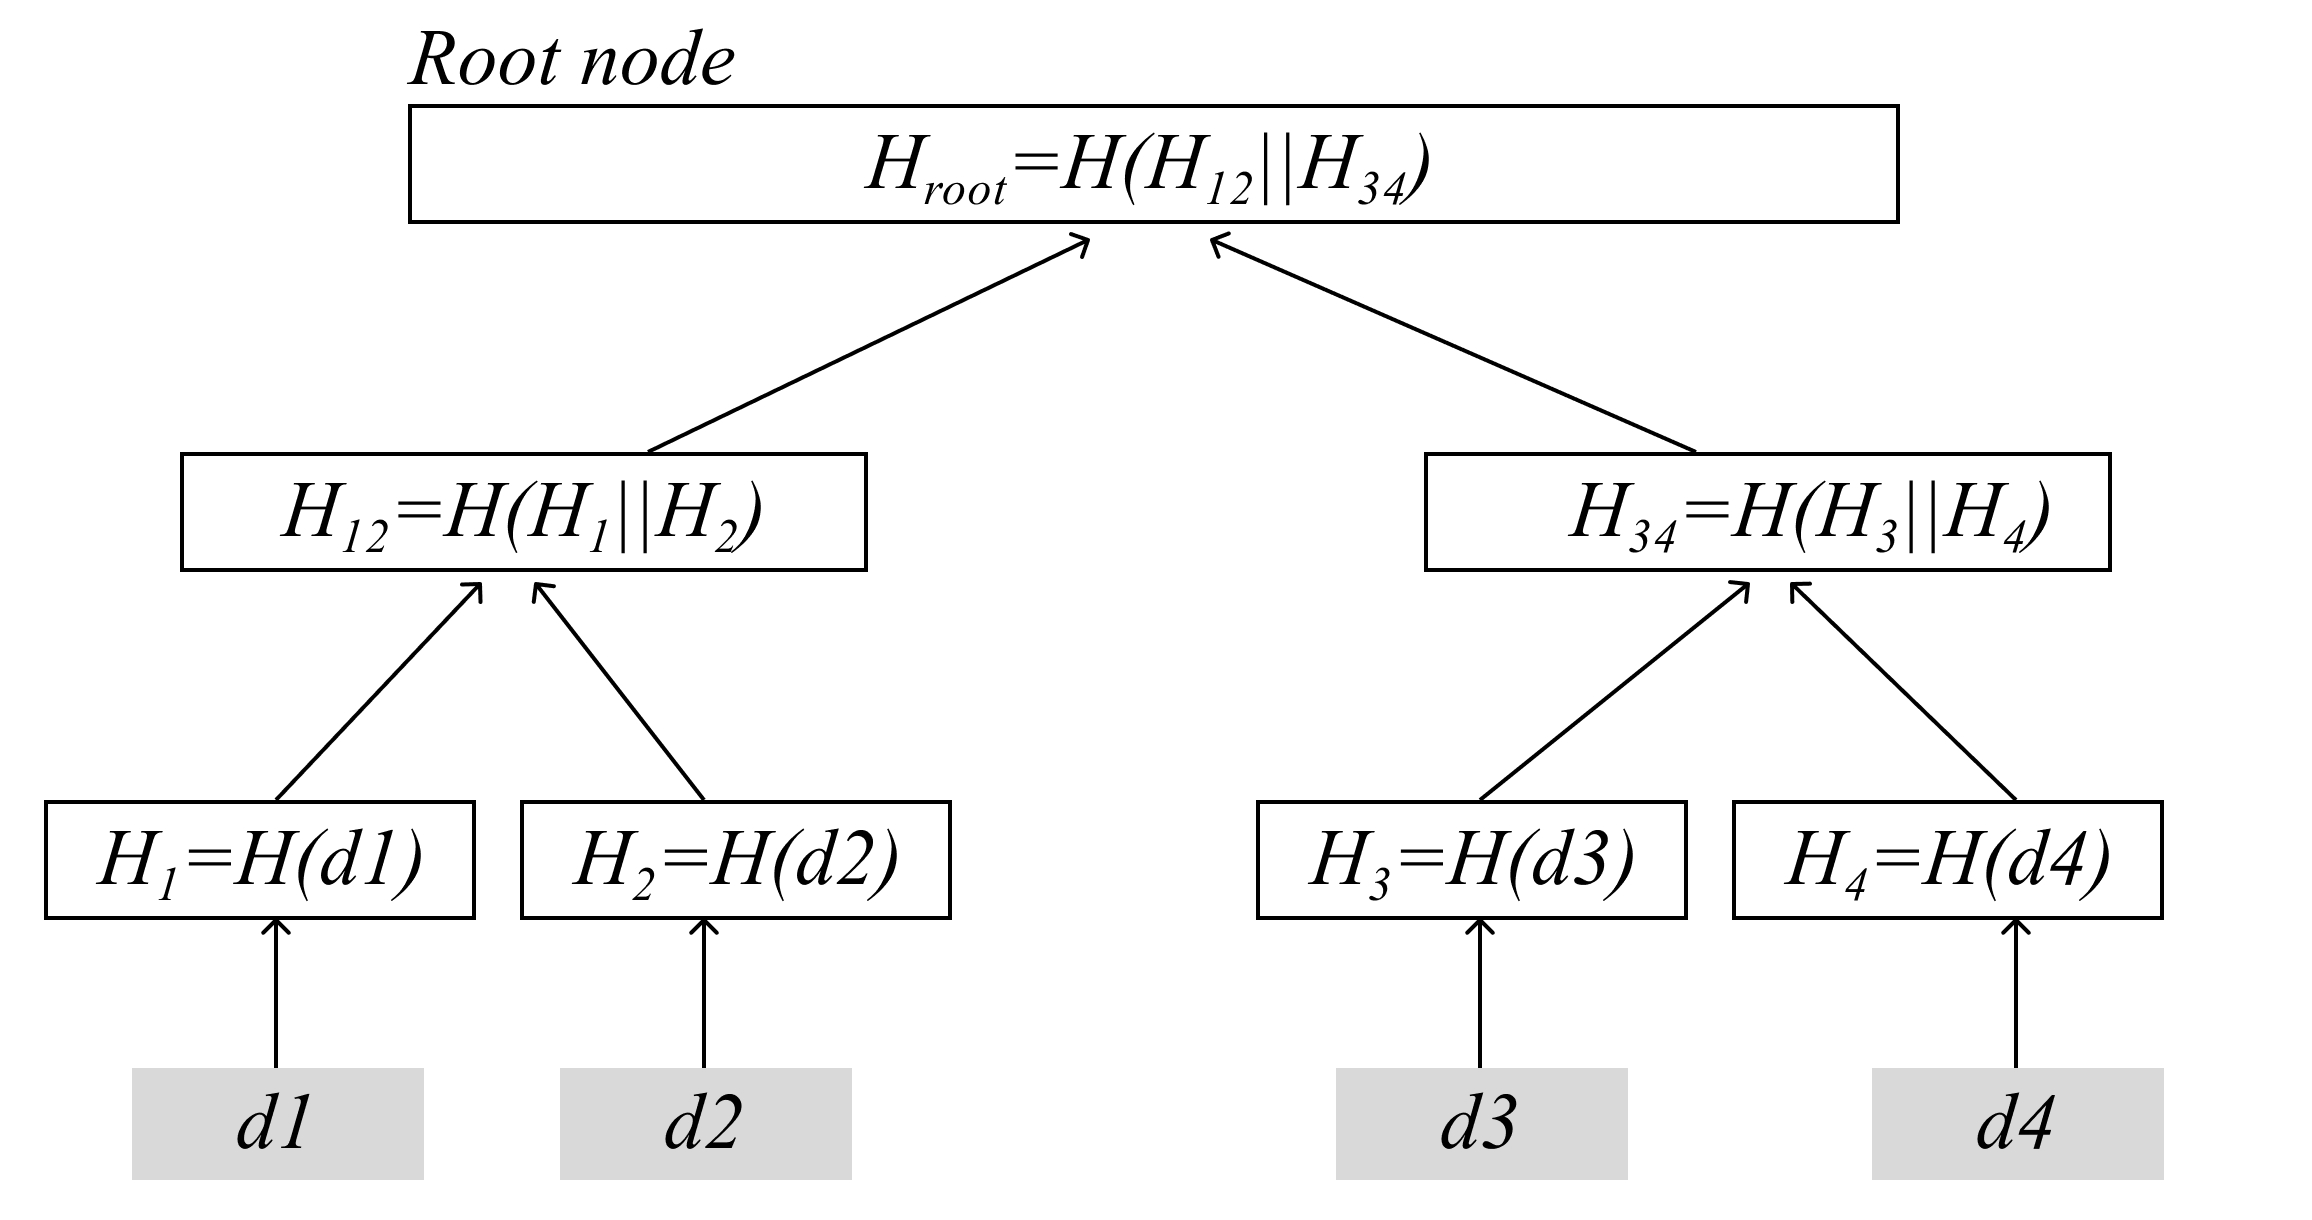
\includegraphics[width=1\textwidth]{Figures/background/merkle_tree.jpg}
  \caption[Merkle tree]{}
  \label{fig:merkle-tree}
\end{figure}

Proving membership of data to a tree with $2^n$ leaves just requires $n$ steps and $n$ intermediate nodes. The algorithm simply reconstructs the tree starting from the node that must be checked, recalculating again the root node. Data is proved to be part of the tree if the recalculated root node is equal to the given root node of the tree.

\subsection{Digital signatures}


\section{The blockchain}

What problem it's solving

\subsection{Double spending problem}

\subsection{Blockchain properties}

\subsection{Consensus layer}

\subsubsection{Proof of work}

\subsubsection{Proof of Stake}

\subsection{51\% attack}

\section{Ethereum}

\subsection{Ethereum as a state machine}

\subsection{Ethereum node}

\subsection{Smart Contracts}

\subsection{EVM}

\subsection{Solidity}

\subsection{ERC20 and ERC721}

% Eventually talk about Dgraph

% section{Graph databases}

% \subsection{Dgraph}



